\section{抽象基类与纯虚函数}
我们在前面讲解继承时一致认为:派生类拥有基类的共性,同时又有自己的独特性。仅用那些共同成员来描述派生类对象是不够的,所以我们需要为派生类添加一些成员,从而更准确地描述派生类的对象。\par
但是实际编程中并不总是如此。有些时候,描述基类对象所需要的成员比描述派生类所需要的成员更多,以致我们不得想办法限制部分成员的值——
\begin{itemize}
    \item 按理,实数应继承自复数(实数是复数的一部分)。但是复数需要至少两个成员(实部和虚部)来表示,而实数只需要一个(实部)。如果我们要写一个 \lstinline@Complex@ 类和一个 \lstinline@Real@ 类,那么必须在继承过程中把 \lstinline@Complex@ 类的虚部成员强制限制为 \lstinline@0@——但这样只会引发无意义的内存空间浪费,我们的 \lstinline@Real@ 类总是存在着一个没有任何作用的成员。
    \item 按理,菱形应继承自平行四边形(各边长相等的平行四边形是菱形)。但是平行四边形需要至少三个成员(两边长及一角)来表示,而菱形只需要两个(一边长及一角)。如果我们要写一个 \lstinline@Parallelogram@ 类和一个 \lstinline@Rhombus@ 类,那么必须在继承过程中把 \lstinline@Parallelogram@ 的两边长成员强制限制为相同值——而且只要改变边长,就必须两个值一起修改。无论怎么说,这也太麻烦了点。
\end{itemize}
面对这样的问题,一种粗糙的处理方式是,把基类与派生类巅倒过来。既然实数只需要一个成员,复数需要两个成员,那么我们就让复数类继承实数类,这不就好了吗?
\begin{lstlisting}
class Real {
    double _r; //共同属于Real和Complex类的实部
};
class Complex : public Real {
    double _i; //专属于Complex类的虚部
}
\end{lstlisting}
这样能解决代码上的困难,但是会造成逻辑上的困惑——复数怎么成了实数的一部分了?读者不要认为这个种属关系只有象征意义就可以乱写,实际上它们的关系会牵扯到很多操作,比如说实数和复数都能取共轭,但只有实数能应用比较运算符。如果我们把复数写成实数的派生类,那么比较运算符这边就很难处理。\par
为了更妥善地解决这个问题,我们需要使用\textbf{抽象基类(Abstract base class, ABC)}。
\subsection*{什么是抽象基类?}
\textbf{抽象类(Abstract class)},简单说来就是不能定义对象的基类。我们曾通过把构造函数写在 \lstinline@protected@ 区或者 \lstinline@private@ 区的做法来防止在类(派生类)外定义对象,但这种做法仍不能避免我们在类内定义对象。抽象类则不同,我们不能在任何地方定义它的对象。与抽象类相对的叫作\textbf{具体类(Concrete class)},我们可以定义它们的对象。\par
抽象类生来就是用来当基类的,所以我们就叫它抽象基类。仍以实数、复数间的关系为例,原本它们是直接继承关系,但如果用直接继承的关系来描述,就会在代码层面引发诸多不便。为此,我们可以把实数和复数的共性(实部)提取出来,作为``抽象复数基类''的成员;然后让复数类和实数类都继承自它,如图10.3所示。\par
\begin{figure}[htbp]
    \centering
    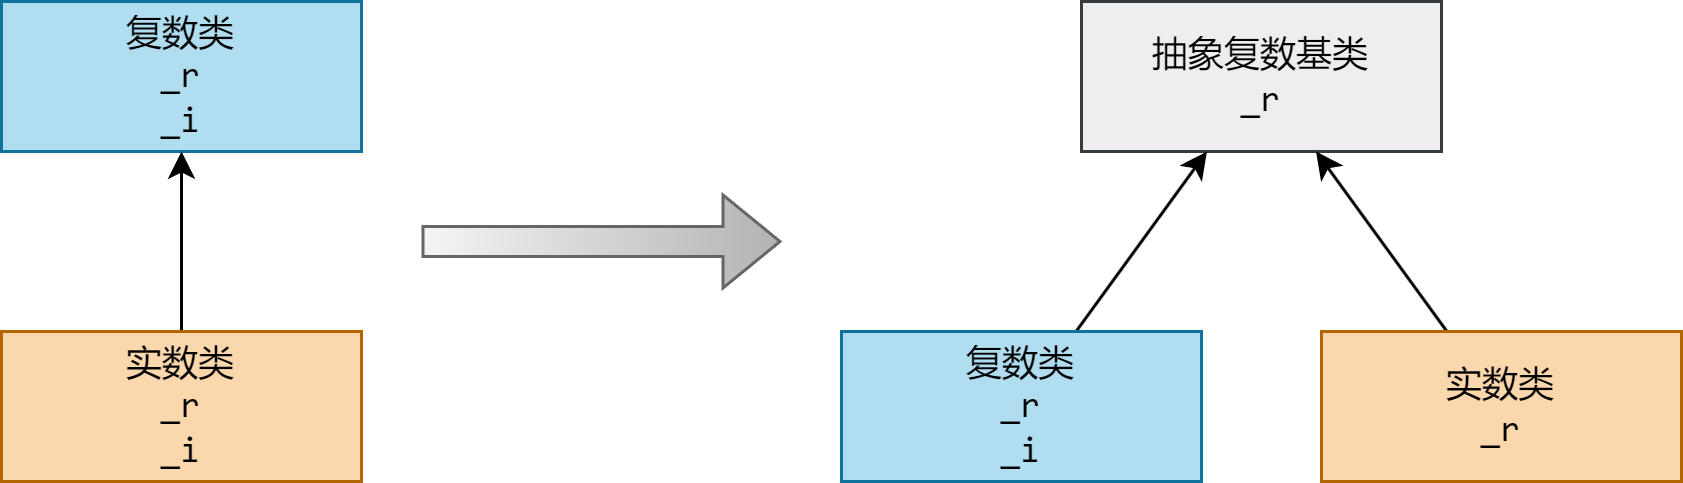
\includegraphics[width=\textwidth]{../images/generalized_parts/10_abstract_complex_class.png}
    \caption{用抽象基类表示 \lstinline@Complex@ 与 \lstinline@Real@ 的关系}
\end{figure}
这样,我们就在保证逻辑关系的条件下避免了让 \lstinline@Real@ 类多出一个 \lstinline@_i@ 成员。\par
对于多级继承的情况来说也可以如此。图10.4就是一个多级继承的例子。\par
\begin{figure}[htbp]
    \centering
    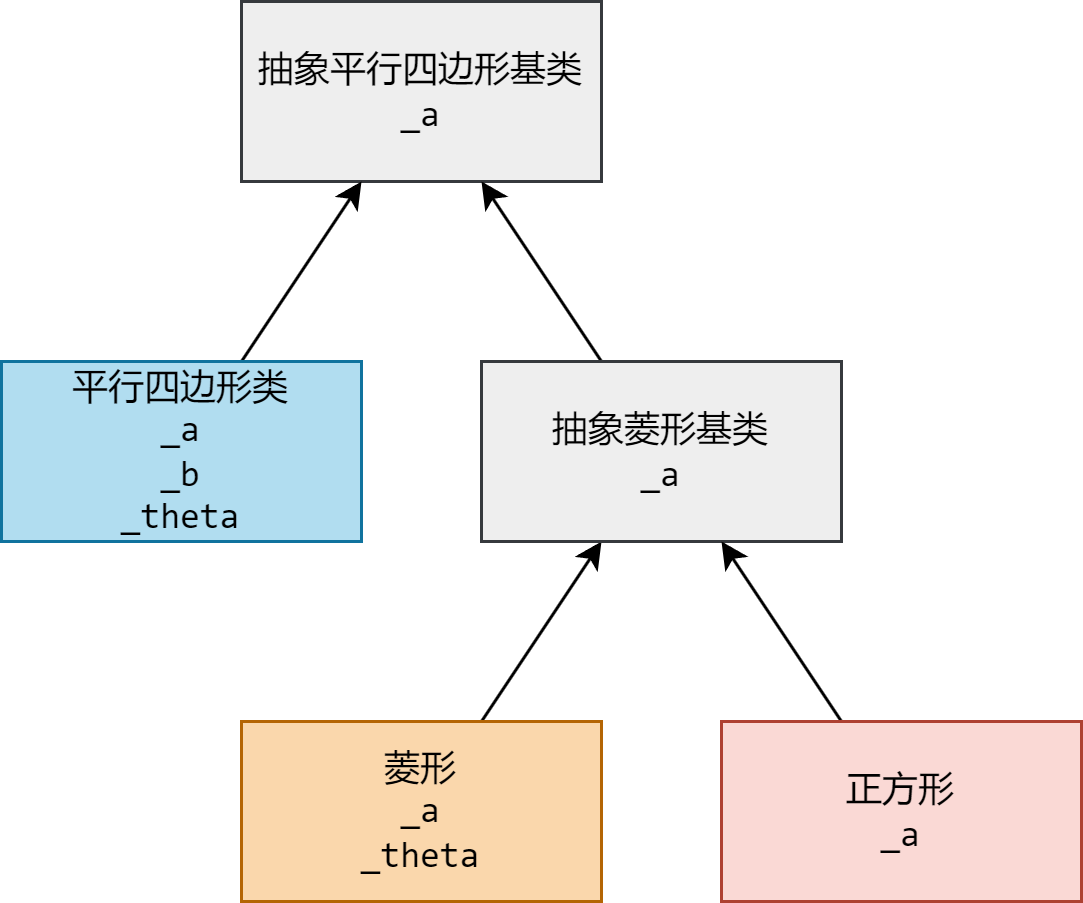
\includegraphics[width=.64\textwidth]{../images/generalized_parts/10_abstract_parallelogram_class.png}
    \caption{用抽象基类表示平行四边形、菱形和正方形的关系}
\end{figure}
\subsection*{纯虚函数}
含有\textbf{纯虚函数(Pure virtual function)}的基类就是抽象基类。\par
我们想,抽象基类没有对象,我们只能用抽象基类的指针/引用来指向其派生类。当调用基类的虚函数时,程序总是能找到对应派生类中的虚函数,并调用之。所以说抽象基类的虚函数没有什么实际作用,它的存在只是为了让编译器不报错——我们讲过,基类指针只能调用基类中声明过的函数;如果只在派生类中声明而未在基类中声明,我们是不能调用的。\par
既然抽象基类的虚函数不可能真的用到,那么我们当然不需要真的给它一个定义。C++中规定,如果给一个虚函数声明添加 \lstinline@=0@ 后缀\footnote{MSVC还支持使用 \lstinline@abstract@ 关键字,不过它不属于C++标准,也未必能在别的编译器中通过编译。},那么这个函数就是纯虚函数,它只有名称意义上存在,而不需要实际意义上的定义。
\begin{lstlisting}
struct Shape { //抽象基类,这个类用来表示各种几何图形
    //...
    virtual double perimeter()const = 0; //周长,纯虚函数
    virtual double area()const = 0; //周长,纯虚函数
};
\end{lstlisting}
抽象基类与纯虚函数之间是充要条件,即:\textbf{只要这个基类中有一个纯虚函数,它就是抽象基类;只要这个基类中没有纯虚函数,它就不是抽象基类。}\par
唯一的特殊情况还是析构函数。一个析构函数无论是不是纯虚函数,它都会被调用。所以我们定义成纯虚函数也没有什么意义,只是给自己找麻烦。因此对于析构函数,我的态度一般是:如果基类中有别的虚函数,那么析构函数最好也要是虚函数;但是析构函数不需要是纯虚函数,那没什么用。\par
\subsection*{实操:不同的几何图形}
接下来我们就用目前为止学到的继承和虚函数方法表示不同几何图形之间的关系,并设计相应的成员函数来计算它们的周长和面积。如有必要,我们也使用抽象基类。\par
为了简便起见,我们只表示三角形、圆形、平行四边形、菱形和正方形。它们都直接或间接继承自 \lstinline@Shape@ 抽象基类,所以我们可以先把这个 \lstinline@Shape@ 写出来。
\begin{lstlisting}
struct Shape { //抽象基类,这个类用来表示各种几何图形
    static constexpr double Pi {3.1415926}; //常量表达式Pi
    static constexpr double Deg2Rad(double deg) { //用于角度转弧度
        return deg * Pi / 180;
    }
    static constexpr double Rad2Deg(double rad) { //用于弧度转角度
        return rad * 180 / Pi;
    }
    virtual double perimeter()const = 0; //周长,纯虚函数
    virtual double area()const = 0; //面积,纯虚函数
};
\end{lstlisting}
这里的 \lstinline@Shape@ 用 \lstinline@struct@ 来定义,这样可以少写一个 \lstinline@public@ 了。\par
接下来我们就用 \lstinline@Shape@ 派生其它类,如图4.5所示。\par
\begin{figure}[htbp]
    \centering
    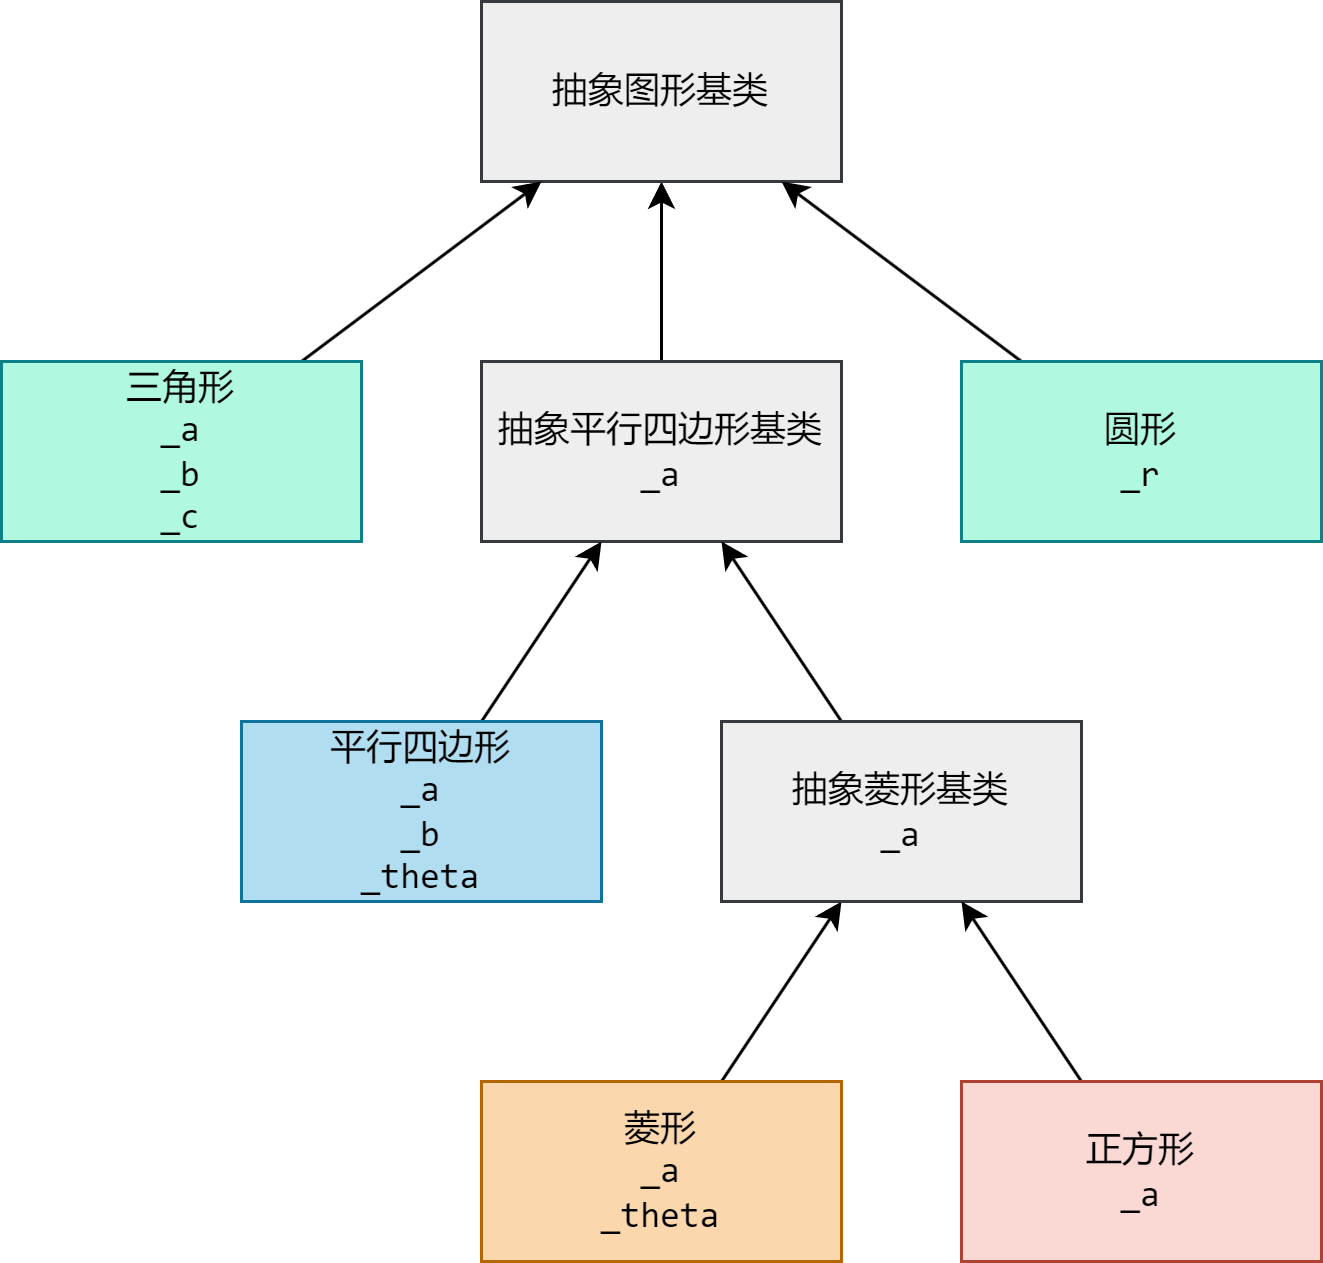
\includegraphics[width=.6\textwidth]{../images/generalized_parts/10_abstract_shape_class.png}
    \caption{\lstinline@Shape@ 之下派生的各个类}
\end{figure}
三角形和圆形的定义很简单,没什么可说的。
\begin{lstlisting}
class Triangle : public Shape { //三角形
    double _a;
    double _b;
    double _c; //三角形的三条边
public:
    Triangle(double a, double b, double c)
        : _a {a}, _b {b}, _c {c} {} //构造函数
    double perimeter()const { return _a + _b + _c; } //周长
    double area()const { //面积
        double s {(_a + _b + _c) / 2};
        return std::sqrt(s * (s - _a) * (s - _b) * (s - _c));
    }
};
class Circle : public Shape { //圆形
    double _r; //圆的半径
public:
    Circle(double r) : _r {r} {}
    double perimeter()const { return 2 * Pi * _r; } //周长
    double area()const { return Pi * _r * _r; } //面积
};
\end{lstlisting}
至于平行四边形这边,就要更复杂一点。我们先把抽象平行四边形基类写出来吧。
\begin{lstlisting}
class Parallelogram_abc : public Shape { // 抽象平行四边形基类
protected:
    double _a; //所有平行四边形都至少需要一条边长信息
public:
    Parallelogram_abc(double a) : _a {a} {} //构造函数
};
\end{lstlisting}
这里我们不需要再写纯虚函数 \lstinline@perimeter@ 和 \lstinline@area@ 了,因为纯虚函数 \lstinline@Shape::perimeter()@ 和 \lstinline@Shape::area()@ 也是 \lstinline@Parallelogram_abc@ 的成员函数。所以 \lstinline@Parallelogram_abc@ 也就自动地变成抽象基类。作为抽象基类,它只有一个属于平行四边形、菱形和正方形的共性,那就是一条边长 \lstinline@_a@。\par
接下来我们定义平行四边形类,它在抽象平行四边形基类的基础上,增加了一条边长和一个角度。
\begin{lstlisting}
    class Parallelogram : public Parallelogram_abc { //平行四边形
    double _b;
    double _theta;
public:
    Parallelogram(double a, double b, double theta)
        : Parallelogram_abc {a}, _b {b}, _theta {theta} {}
    double perimeter()const { return 2 * (_a + _b); }
    double area()const { return _a * _b * std::sin(Deg2Rad(_theta)); }
};
\end{lstlisting}
这里的周长和面积仍然是虚函数,但是我们不用把 \lstinline@virtual@ 写出来。在 \lstinline@Parallelogram@ 的构造函数函数中,\lstinline@_a@ 的初始化要交给 \lstinline@Parallelogram_abc@ 来完成。这也就意味着,虽然我们不能定义抽象基类的对象,但是调用抽象基类的构造函数还是有可能的。\par
接下来是抽象菱形基类的定义。
\begin{lstlisting}
struct Rhombus_abc : Parallelogram_abc { //抽象菱形基类
    Rhombus_abc(double a) : Parallelogram_abc {a} {} //构造函数
};
\end{lstlisting}
这里我们不需要添加新的成员对象,只需要写一个构造函数就够了。至于纯虚函数,它可以继承自 \lstinline@Parallelogram_abc@,我们无须再写。\par
下面分别定义菱形和正方形类就可以了,很简单。
\begin{lstlisting}
class Rhombus : public Rhombus_abc { //菱形
    double _theta;
public:
    Rhombus(double a, double theta) : Rhombus_abc {a}, _theta {theta} {}
    double perimeter()const { return 4 * _a; }
    double area()const { return _a * _a * std::sin(Deg2Rad(_theta)); }
};
struct Square :  Rhombus_abc { //正方形
    Square(double a) : Rhombus_abc {a} {}
    double perimeter()const { return 4 * _a; }
    double area()const { return _a * _a; }
};
\end{lstlisting}
我们突然发现,\lstinline@Rhombus::perimeter()@ 和 \lstinline@Square::perimeter()@ 的定义是完全相同的——实际上菱形与正方形的周长公式真的完全一致。因此我们还可以把它们作为共性,定义到抽象菱形基类当中,也就是把上述代码改成这样:
\begin{lstlisting}
struct Rhombus_abc : Parallelogram_abc { //抽象菱形基类
    double perimeter()const { return 4 * _a; }
    Rhombus_abc(double a) : Parallelogram_abc {a} {} //构造函数
};
class Rhombus : public Rhombus_abc { //菱形
    double _theta;
public:
    Rhombus(double a, double theta) : Rhombus_abc {a}, _theta {theta} {}
    double area()const { return _a * _a * std::sin(Deg2Rad(_theta)); }
};
struct Square : Rhombus_abc { //正方形
    Square(double a) : Rhombus_abc {a} {}
    double area()const { return _a * _a; }
};
\end{lstlisting}
而当调用 \lstinline@Rhombus@ 或者 \lstinline@square@ 的 \lstinline@perimeter()@ 函数时,编译器自然能根据名称查找规则找到 \lstinline@Rhombus_abc::perimeter()@ 来。总而言之,不必为此操心。\par
